\documentclass[conference]{IEEEtran}
\IEEEoverridecommandlockouts
% The preceding line is only needed to identify funding in the first footnote. If that is unneeded, please comment it out.
\usepackage{cite}
\usepackage{amsmath,amssymb,amsfonts}
\usepackage{algorithmic}
\usepackage{graphicx}
\usepackage{textcomp}
\usepackage{xcolor}

\begin{document}
	
	\title{Received Signal Strength Indicator and Its Analysis
		in a Typical WLAN System (Short Paper)\\
		{\footnotesize \textsuperscript{*}Note:Yogita Chapre ∗§, Prasant Mohapatra†
			, Sanjay Jha∗
			and Aruna Seneviratne ‡§
			∗School of Computer Science & Engineering, University of New South Wales, Sydney, Australia
			†Department of Computer Science, University of California, Davis, CA 95616
			‡School of Electrical Engineering & Telecommunications, University of New South Wales, Australia
			§ Networks Research Group, NICTA, Sydney, Australia
			Email: {yogitac, sanjay}@cse.unsw.edu.au, prasant@cs.ucdavis.edu, {yogita.chapre, aruna.seneviratne}@nicta.com.au }
		\thanks{Identify applicable funding agency here. If none, delete this.}
	}
	
	
	\maketitle
	
	\begin{abstract}
		Received signal strength based fingerprinting approaches have been widely exploited for localization. The received
		signal strength (RSS) plays a very crucial role in determining
		the nature and characteristics of location fingerprints stored in a
		radio-map. The received signal strength is a function of distance
		between the transmitter and receiving device, which varies due
		to various in-path interferences. A detailed analysis of factors
		affecting the received signal for indoor localization is presented
		in this paper. The paper discusses the effect of factors such as
		spatial, temporal, environmental, hardware and human presence
		on the received signal strength through extensive measurements
		in a typical IEEE 802.11b/g/n network. It also presents the
		statistical analysis of the measured data that defines the reliability
		of RSS-based location fingerprints for indoor localization.
	\end{abstract}
	
	\begin{IEEEkeywords}
		component, formatting, style, styling, insert
	\end{IEEEkeywords}
	
	\section{Introduction}
	Historically, received signal strength indicator (RSSI) based
	fingerprinting has been playing a key role in numerous indoor
	positioning systems. Typical location fingerprinting algorithms
	consist of two phases: an off-line/training phase and an online/positioning phase. The training phase consists of collection of RSSI at known distinct locations called as Reference
	Points (RPs). These RPs are stored as a fingerprint in a radiomap. In the positioning phase, real-time data is collected
	at an unknown location called as a Test Point (TP). The
	localization algorithm uses the radio-map to derive the location
	of a TP by calculating the Euclidean distance between a
	TP and each RP fingerprint. The fingerprint consists of N
	RSS values for each cited Beacon/Access Point (AP) in a
	wireless network. Furthermore, localization algorithm uses
	either probabilistic or deterministic methods for positioning
	[1] [2]. RSS as a fingerprint forms a basis in creating a radiomap for fingerprinting algorithms.
	RSS at a given location is average of the signal received
	through different paths (multipath effects). Therefore, it becomes crucial to determine the factors that affect RSS. In this
	paper, we attempt to answer the question, whether RSSI can be
	used for creating the reliable location fingerprints? The main
	objective of our experiment is to study the characteristics of
	the RSS, to figure out the parameters and its effect on the RSS
	at a particular location and instant of time. We investigate the
	effects of hardware orientation, location, time and duration of
	measurement, interference and user’s presence on the RSS
	
	\section{Related Work}
	
The data analysis of localization algorithm has been presented in [1]- [3]. Bahl et al. presents the effect of user’s
orientation on the mean value of RSS [1]. The study shows
that RSS at a location can deviate by 5 dBm maximum
depending on user’s orientation. Based on the observations,
researchers have suggested to exploit the orientational database
for fingerprinting to improve the accuracy of localization. In
[3] authors have pointed out that the factors such as hardware
quality and number of received samples from APs affects the
localization. But the study have not presented any investigations regarding the effect of these factors on localization.
Ahmad et al. presented the analysis of the temporal variations
on RSS samples [4]. The study indicates that the absence of
samples from APs due to degradation of radio channels may
adversely affect the indoor localization. This can degrade the
performance and scalability of the localization algorithm with
more computations. In [5] author has presented the detailed
analysis of RSSI measurement and investigated the effect of
wireless local area network (WLAN) card, time and duration
of measurement, interference and building environment (corridor, small office or large hall). Make of WLAN card affects
RSS significantly due to different quantization bins. However,
the effect of user’s presence and device orientation on RSSI
is not considered. Further the study considers the antenna of
WLAN card to be omni-directional. The analysis in carried out
in 3 different building environment using limited (maximum
6) APs.
All these studies raised some serious concerns on reliability
of the RSSI in fingerprinting. In our studies, we show empirically that the RSSI is significantly affected by hardware orientation and several other factors. Therefore, RSSI when used to
create location signatures are unreliable when multiple devices
from different vendors and physical constraints are being used.
However it may be possible to use RSSI for fingerprinting
using a single device with fixed hardware configuration to
provide the reliable location fingerprints.

	
\section{Data Analysis}
In this section, we present the details regarding our measurements, figure out the various contributing factors responsible
for RSS variation and discuss the statistical properties of the
measured data.
	\subsection{Measurement Data Summary}
	The summary of logged data is shown in Table I
	
	\begin{table}[htbp]
		\caption{Table Type Styles}
		\begin{center}
			\begin{tabular}{|c|c|c|c|}
				\hline
				\textbf{Location}&\multicolumn{3}{|c|}{\textbf{Factors}} \\
				\cline{2-4} 
				\textbf{Head} & \textbf{\textit{Duration in days}}& \textbf{\textit{total samples}}& \textbf{\textit{observerd}} \\
				\hline
				Location 1& 2&66306&84$^{\mathrm{a}}$& &  \\
				\hline
				
				Location 2& 4&67306&67$^{\mathrm{a}}$& &  \\
				\hline
				\multicolumn{4}{l}{$^{\mathrm{a}}$Sample of a Table footnote.}
			\end{tabular}
			\label{tab1}
		\end{center}
	\end{table}
	
	\begin{figure}[htbp]
		\centerline{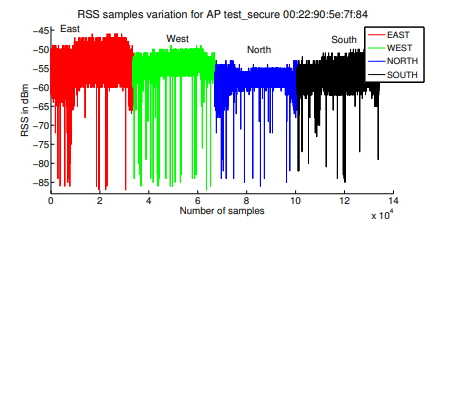
\includegraphics{fig1.png}}
		\caption{RSSI for different orientations}
		\label{fig}
	\end{figure}
	
	\section{Conclusion}
	In this paper, we have investigated the factors affecting
	RSS including orientation of the receiver, distance between
	transmitter and receiver, time and duration of measurement,
	interference due to other radio devices, presence of human and
	building environment on the RSSI. We had shown empirically
	that the RSSI fluctuations are quite significant even for a
	single hardware. In the case of multiple devices from different
	vendors are used, this variations will be amplified even further
	due to different sampling rates and quantization bins. Our
	experiment shows that diferent orientation of a single device
	results in at least 2 dBm mean deviation whereas location
	granularity of 1 meter leads to upto 6 dBm mean fluctuation.
	Further, time and duration of the measurement for determining
	the required number of samples to form a location fingerprint
	varies due to irregularity of samples, its distribution and skewness. From our analysis, it is evident that multiple orientations
	at a fixed location with user’s presence can provide various
	radio signatures that can be incorporated in the radio-map
	for location fingeprinting. We intend to explore the possibility
	of exploiting aggregated information from different types of
	devices, to determine the correlation between different devices
	that results in RSSI variation. This will help in normalizing
	the hardware dependency to provide more robust location
	fingerprinting using RSS signatures.
	References
	
	
	
	\begin{thebibliography}{00}
		\bibitem{b1} P. Bahl and V. Padmanabhan, “RADAR: an in-building RF-based user
		location and tracking systems,” in Proceedings INFOCOM00’: Nineteenth
		Annual Joint Conference of the IEEE Computer and Communications
		Societies. IEEE, vol. 2, 2000, pp. 775–784.
		\bibitem{b2} M. Youssef and A. Agrawala, “The Horus WLAN location determination
		system,” in MobiSys’05: Proceedings of the 3rd international conference
		on Mobile systems, applications and services, USA, 2005, pp. 205–218.
		\bibitem{b3} H. Lemelson, T. King, and W. Effelsberg, “Pre-processing of fingerprints
		to improve the positioning accuracy of 802.11-based positioning systems,”
		in MELT ’08: Proceedings of the first ACM international workshop on
		Mobile entity localization and tracking in GPS-less environments, San
		Francisco, California, USA, 2008, pp. 73–78.
		
	\end{thebibliography}
	
	
\end{document}
